\chapter{Testbed setup}
\label{cha:testbed}

In this section, we will illustrate how we set up a \textbf{testbed} with ComNetsEmu to evaluate the performance of \textbf{low-latency adaptive bitrate live streaming} technologies. The testbed allows to run experiments in different scenarios and configurations, extracting some important metrics and events that are then used for analysis. 

We will then use this testbed to evaluate the performance of some existing streaming technologies (Chapter \ref{cha:eval}) and to propose some improvements (Chapter \ref{cha:improvements}).

\section{General architecture}
\label{sec:testbed/architecture}

The testbed for evaluating the quality of experience (QoE) of live streaming solutions was built with ComNetsEmu. The project was published as an open source project at \url{https://github.com/matteocontrini/live-streaming-testbed}.

The general architecture of the testbed is shown in Figure X. The topology of the emulated network consists of three hosts (H1, H2, H3) and two switches (S1, S2). The link between the two switches represents an unreliable network such as an Internet access network. When the emulation is run, a series of experiments with different configurations are run, and the link parameters are changed. For example, the bandwidth is varied to emulate a real network with oscillating throughput.

\begin{figure}[h]
    \centering
    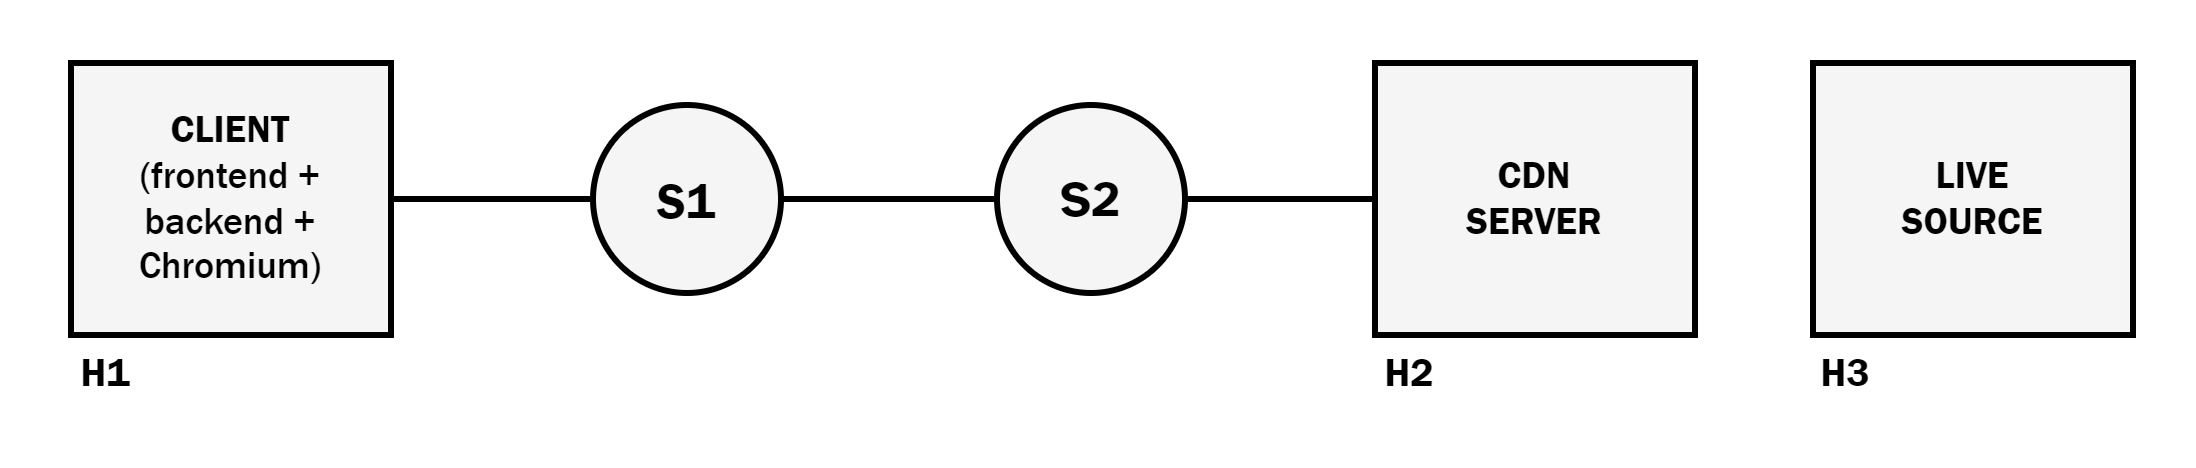
\includegraphics[width=\textwidth]{res/testbed.png}
    \caption{Diagram of the testbed architecture, based on ComNetsEmu.}
    \label{fig:testbed}
\end{figure}

On the three hosts, several applications are deployed as Docker containers.

\begin{itemize}
    \item \texttt{H3} hosts a script that performs the \textbf{packaging of a live stream} in both HLS and DASH formats. It runs an \ffmpeg{} command that simulates a live stream, taking an MP4 file as input. The output of this application, called \textit{live source}, are manifest and playlist files for both HLS and DASH and the corresponding video and audio segments in \texttt{fMP4} format.
    \item \texttt{H2} acts as an \textbf{HTTP CDN server} for the packaged stream. In practice, it is an \texttt{h2o} web server that serves the files produced by the live source, over HTTP/1.1, HTTP/2 and HTTP/3. It also takes care of provisioning the public key certificates that are required for HTTPS.
    \item \texttt{H1}, which is on the other side of the main network link, is the client. It consists of a frontend application containing a \textbf{video player} that plays the live video stream generated by the server. The frontend application also takes care of collecting several metrics from the player and transmitting them to a Node.js backend application. The frontend application runs in a \textbf{Chromium headless} instance, which is started by the backend application through the \textbf{Puppeteer} library.
\end{itemize}

To start the emulation through ComNetsEmu, one first needs to clone the source code of the testbed. The ABR video renditions should then be encoded and written in an MP4 file, which the live source will then use to simulate the live stream (we will see this in detail in Section \ref{sec:testbed/packaging}). To start the Vagrant virtual machine and start a session, the following commands can be used.

\begin{minted}[frame=single]{bash}
vagrant up
vagrant ssh
\end{minted}

Finally, after building the Docker images, the emulation can be started, as shown in the following code block. The testbed source code actually contains scripts that can be used to execute these commands more easily. They also handle error handling and cleanup.

\begin{minted}[frame=single]{bash}
cd live-source && docker build -t live-source .
cd ../cdn && docker build -t cdn .
cd ../client && docker build -t client .
cd .. && sudo python3 topology.py
\end{minted}

Before going into the details of how the specific components were developed, it should be noted that the default Vagrant configuration for ComNetsEmu (contained in a file known as \texttt{Vagrantfile}) does not work when the machine architecture is ARM. This is especially problematic on newer laptops that use Apple Silicon hardware, such as the M1 and M2 chips.

To solve this problem, two changes must be applied to the ComNetsEmu \texttt{Vagrantfile}. First, the Vagrant box (the operating system image) must be changed to an image that is built for the ARM architecture. Then, since x86 virtualization software such as VirtualBox cannot be used on ARM systems, a new virtual machine provider must be added. In practice, for Mac systems, this means enabling Parallels Desktop as a virtual machine provider. Figure \ref{fig:vagrantfile} shows how the \texttt{Vagrantfile} of ComNetsEmu was modified for Apple Silicon support.

\begin{figure}
    \centering
    \begin{minted}[frame=single,linenos,fontsize=\small]{diff}
diff --git a/Vagrantfile b/Vagrantfile
index 0f07076..a21824f 100644
--- a/Vagrantfile
+++ b/Vagrantfile
@@ -20,6 +20,8 @@ VM_NAME = "ubuntu-20.04-comnetsemu"
 # When using libvirt as the provider, use this box, bento boxes do not support...
 BOX_LIBVIRT = "generic/ubuntu2004"

+BOX_PARALLELS = "jeffnoxon/ubuntu-20.04-arm64"
+
 ######################
 #  Provision Script  #
 ######################
@@ -105,6 +107,14 @@ Vagrant.configure("2") do |config|
     # Sync ./ to home directory of vagrant to simplify the install script
     comnetsemu.vm.synced_folder ".", "/vagrant", disabled: true
     comnetsemu.vm.synced_folder ".", "/home/vagrant/comnetsemu"
+
+    # Parallels Desktop
+    config.vm.provider "parallels" do |prl, override|
+      override.vm.box = BOX_PARALLELS
+      prl.name = VM_NAME
+      prl.cpus = CPUS
+      prl.memory = RAM
+    end

     # For Virtualbox provider
     comnetsemu.vm.provider "virtualbox" do |vb|
    \end{minted}
    \caption{Diff showing how the ComNetsEmu \texttt{Vagrantfile} was modified to add support for Apple Silicon machines.}
    \label{fig:vagrantfile}
\end{figure}


\section{Live stream generation and packaging}
\label{sec:testbed/packaging}

To avoid having an actual live source such as a camera, the live video stream was simulated. There are multiple ways to simulate a live video stream. For example, there exist several streaming servers that handle video ingestion, transcoding and packaging. For our testbed, we chose to implement a simpler solution based on \ffmpeg{} and a static input video file.

In fact, since we do not need the live stream to be dynamic, we decided to encode the video renditions beforehand. The renditions are then packaged as live streams each time the emulation is run, as if they were ingested and transcoded live. This solution makes the test setup much lighter in terms of computational resources, with a similar result.

When encoding the video renditions, we chose the following bitrate ladder. All video renditions are encoded with H.264 at 25 fps with a keyframe/I-frame interval of 2 seconds and a constant bitrate.

\begin{itemize}
    \item \texttt{1280x720} at 3.5 Mbps;
    \item \texttt{960x540} at 2.5 Mbps;
    \item \texttt{640x360} at 1.5 Mbps;
    \item \texttt{480x720} at 0.8 Mbps.
\end{itemize}

The audio is instead encoded with \texttt{AAC-LC} at 128 kbps. Of course, there are many other possible configurations, but the above is a common configuration that gives good quality results.\cite{ozer}

The \ffmpeg{} command that was used to produce the renditions is similar to the following:

\begin{minted}[frame=single,fontsize=\small]{bash}
ffmpeg -i $INPUT \
  -c:v libx264 -pix_fmt yuv420p -preset veryfast -r 25 \
  -g 50 -keyint_min 50 -sc_threshold 0 \
  -force_key_frames 'expr:gte(t,n_forced*2)' -refs 1 \
  -c:a libfdk_aac -ac 2 -b:a 128k \
  -map 0:a:0 -map 0:v:0 -map 0:v:0 -map 0:v:0 -map 0:v:0 \
  -s:v:0 1280x720 -b:v:0 3500k -bufsize:v:0 3500k -minrate:v:0 3500k -maxrate:v:0 3500k \
  -s:v:1 960x540 -b:v:1 2500k -bufsize:v:1 2500k -minrate:v:1 2500k -maxrate:v:1 2500k \
  -s:v:2 640x360 -b:v:2 1500k -bufsize:v:2 1500k -minrate:v:2 1500k -maxrate:v:2 1500k \
  -s:v:3 480x270 -b:v:3 800k -bufsize:v:3 800k -minrate:v:3 800k -maxrate:v:3 800k \
  abr.mp4
\end{minted}

In detail, the meaning of the options is as follows.

\begin{itemize}
    \item \texttt{-i} specifies the input media file, which can be in any format supported by \ffmpeg{}.
    \item \texttt{-c:v} specifies the video codec, in this case \texttt{libx264}, a library that implements x264 (a popular open source software-based H.264 encoder).
    \item \texttt{-pix\_fmt} defines the pixel format. A value of \texttt{yuv420p} means that the pixels are encoded with Y'CbCr 4:2:0 chroma subsampling.
    \item \texttt{-preset} specifies a set of configuration options that influence which H.264 features are used and thus the encoding speed. Research has shown that \texttt{veryfast} is a good trade-off between speed and quality.\cite{ozer}
    \item \texttt{-r} sets the \textit{frames per second} (fps) value. In this case, 25 fps are used.
    \item \texttt{-g} and \texttt{-keyint\_min} tell the encoder the maximum and minimum GOP size in frames, that is, the minimum and maximum interval between key frames (I-frames).
    \item \texttt{-sc\_threshold} adjusts a parameter for scene cut detection, which is an algorithm that analyzes the difference between frames to determine whether a new I-frame should be inserted due to a scene change. Setting the parameter to 0 means that scene detection is disabled. This is a common choice when encoding for streaming, since I-frames are very expensive compared to other frame types.\cite{ozer}
    \item \texttt{-force\_key\_frames} forces a key frame when the given expression evaluates to \texttt{true} at the current frame. This option is required because \texttt{x264} does not allow setting \texttt{-keyint\_min} to a value greater than \texttt{keyint/2+1}, and clips the value if it is larger.\footnote{\url{https://github.com/mirror/x264/blob/b093bbe7d9bc642c8f24067cbdcc73bb43562eab/encoder/encoder.c\#L1111}} The expression \texttt{gte(t,n\_forced*2)} means that a keyframe should be forced every 2 seconds (in the expression, \texttt{t} is the time of the current frame and \texttt{n\_forced} is the number of frames forced so far).
    \item \texttt{-refs} specifies the number of reference frames that each inter-predicted frame can use. Research has shown that limiting the number of frames to 1 has a negligible impact on quality while reducing the encoding time.\cite{ozer}
    \item \texttt{-c:a} specifies the audio codec, in this case \texttt{libfdk\_aac}, a high-quality AAC implementation by the Fraunhofer research institute.
    \item \texttt{-ac} specifies the number of audio channels, 2 in this case (stereo).
    \item \texttt{-b:a} specifies the audio bitrate, which is constant (CBR) by default.
    \item \texttt{-map} is used to select which streams of the input file should be sent to the output. For example, \texttt{-map 0:a:0} takes the first audio track from the first input file and includes it in the output file. Multiple \texttt{-map} options for the same input stream have the effect of duplicating the stream. In this case, we use \texttt{-map} to create multiple video streams (one per rendition), within a single command.
    \item \texttt{-s:v} is used to scale the video to the specified resolution. In our command, this option is used once per rendition to change the resolution for reach of the (duplicated) video streams.
    \item \texttt{-b:v}, \texttt{-minrate:v}, \texttt{-maxrate:v}, \texttt{-bufsize:v} set the average target bitrate, the minimum bitrate, the maximum bitrate, and the buffer size of the encoder. By setting all the options to the same value the result is a constant bitrate (CBR) video stream, which is often recommended for adaptive bitrate streaming and helps to comply with Apple HLS Authoring Specification.\cite{ozer}\cite{hlsauthoring}
\end{itemize}

\texttt{ffmpeg} will choose the appropriate \textbf{H.264 profile and level} based on the selected preset and the other encoding parameters. In our case, the profile will be set to \texttt{High} for all the renditions, while the level varies between 2.1 and 3.1 depending on the resolution and bitrate.

The output generated by the command is a single MP4 file that contains multiple tracks, one per each video rendition and one for the audio, as shown in Figure \ref{fig:ffprobe_abr}.

\begin{figure}[h]
    \centering
    \begin{minted}[frame=single,breaklines,fontsize=\footnotesize]{text}
Input #0, mov,mp4,m4a,3gp,3g2,mj2, from 'abr.mp4':
  Metadata:
    major_brand     : isom
    minor_version   : 512
    compatible_brands: isomiso2avc1mp41
    title           : Big Buck Bunny, Sunflower version
    artist          : Blender Foundation 2008, Janus Bager Kristensen 2013
    composer        : Sacha Goedegebure
    encoder         : Lavf59.31.100
    comment         : Creative Commons Attribution 3.0 - http://bbb3d.renderfarming.net
    genre           : Animation
  Duration: 00:10:34.64, start: 0.000000, bitrate: 7884 kb/s
  
  Stream #0:0[0x1](und): Audio: aac (LC) (mp4a / 0x6134706D), 48000 Hz, stereo, fltp, 128 kb/s (default)
  
  Stream #0:1[0x2](und): Video: h264 (High) (avc1 / 0x31637661), yuv420p(progressive), 1280x720 [SAR 1:1 DAR 16:9], 3238 kb/s, 25 fps, 25 tbr, 12800 tbn (default)
  
  Stream #0:2[0x3](und): Video: h264 (High) (avc1 / 0x31637661), yuv420p(progressive), 960x540 [SAR 1:1 DAR 16:9], 2341 kb/s, 25 fps, 25 tbr, 12800 tbn (default)
  
  Stream #0:3[0x4](und): Video: h264 (High) (avc1 / 0x31637661), yuv420p(progressive), 640x360 [SAR 1:1 DAR 16:9], 1409 kb/s, 25 fps, 25 tbr, 12800 tbn (default)
  
  Stream #0:4[0x5](und): Video: h264 (High) (avc1 / 0x31637661), yuv420p(progressive), 480x270 [SAR 1:1 DAR 16:9], 751 kb/s, 25 fps, 25 tbr, 12800 tbn (default)
  
    \end{minted}
    \caption{\texttt{ffprobe}'s output showing the 5 video tracks of the ABR MP4 file. Some metadata was omitted for brevity.}
    \label{fig:ffprobe_abr}
\end{figure}

When the emulation starts, one of the applications that is executed is the live source, which in practice is the HLS and DASH packager. This is again a \ffmpeg{} script, run inside a Docker container. The script takes the previously generated MP4 file as input and generates \texttt{fMP4} chunks (for each rendition), plus HLS playlists and the DASH manifest.

The \ffmpeg{} command used for packaging is similar to the following:

\begin{minted}[frame=single]{bash}
ffmpeg -re -i $SOURCE \
  -map 0 -c copy \
  -utc_timing_url 'https://time.akamai.com/?iso' \
  -seg_duration 2 \
  -dash_segment_type mp4 \
  -use_template 1 -use_timeline 0 \
  -init_seg_name 'init-stream-$RepresentationID$.m4s' \
  -media_seg_name 'chunk-stream-$RepresentationID$-$Number%05d$.m4s' \
  -adaptation_sets 'id=0,streams=v id=1,streams=a' \
  -hls_playlist 1 \
  -f dash \
  $OUT_DIR/manifest.mpd
\end{minted}

Specifically, the meaning of the arguments and options is as follows.

\begin{itemize}
    \item \texttt{-re} limits the read rate so that it aligns with the frame rate. Without this option, \ffmpeg{} would read the whole video without respecting the playback rate.
    \item \texttt{-c} with a value of \texttt{copy} tells \ffmpeg{} to copy the input streams without re-encoding, since we have already encoded them previously.
    \item \texttt{-utc\_timing\_url} defines the URL of a web page that returns the current UTC timestamp in ISO format. This is required by DASH on the client side for time synchronization.
    \item \texttt{-seg\_duration} specifies the duration of each segment/fragment that is generated. For better performance, segments should start with a key frame, which is the reason why we set the value at 2 seconds, corresponding to the GOP length of the input file.
    \item \texttt{-dash\_segment\_size} with a value of \texttt{mp4} specifies that the packer should output CMAF-compliant \texttt{fMP4} segments.
    \item \texttt{-use\_template} and \texttt{-use\_timeline} enable the use of DASH \texttt{SegmentTemplate} to avoid listing all the video segments in the manifest. This is possible because the segments have a fixed duration.
    \item \texttt{-init\_seg\_name} and \texttt{-media\_seg\_name} define the file name format for the initialization segment and the individual media segments.
    \item \texttt{-adaptation\_sets} specifies which adaptation sets should be added to the DASH manifest. The expression \texttt{id=0,streams=v id=1,streams=a} defines two adaptation sets, one with all the video streams (ID 0) and the other one 
    with the audio stream (ID 1).
    \item \texttt{-hls\_playlist 1} specifies that the DASH muxer should also generate HLS playlists, using the same \texttt{fMP4} segments. The packager will create a \texttt{master.m3u8} file for the master playlist and a set of media playlists with file names \texttt{media\_0.m3u8}, \texttt{media\_1.m3u8}, etc.
    \item \texttt{-f dash} sets the \ffmpeg{} output muxer to DASH.
    \item Finally, the path of the DASH manifest file (\texttt{.mpd}) is specified.
\end{itemize}

The output of the package are the \texttt{fMP4} files, the DASH manifest and the HLS manifest. These are put in a Docker-mounted directory, which is shared with the CDN container.

\section{CDN server}
\label{sec:testbed/cdn}

The "CDN" part of the setup consists of the \texttt{h2o} HTTP server, an open source software maintained by Fastly developers. \texttt{h2o} is built from source during the initial creation of the Docker images, since we are using a fork of \texttt{h2o} with some modifications.

The web server is configured to listen on three separate ports for HTTP/1.1, HTTP/2 and HTTP/3, therefore making it possible to test the three protocols independently. As we shall see, instead of relying on the \texttt{Alt-Svc} HTTP header to inform the browser about the availability of HTTP/3 on a specific port, we will configure the browser to force HTTP/3 on the corresponding port from the beginning, avoiding upgrades from other protocols.

With respect to HTTP/2, a problem we encountered was the inability to tell \texttt{h2o} to enable/disable HTTP/2 only on a specific port. However, since HTTP/2 only works over TLS, the workaround was to use port 80 for HTTP/1.1 and port 443 for HTTP/2. This approach works because this configuration only allows HTTP/1.1 to be used on port 80, while on port 443 the connection is started with TLS and HTTP/2 is used. The browser knows that it should use HTTP/2 and not HTTP/1.1 over port 443 thanks to a TLS feature, called \textbf{Application-Layer Protocol Negotiation} (ALPN), which allows negotiation of the HTTP version during the TLS handshake.

In \texttt{h2o}, HTTP/3 must instead be explicitly enabled on a specific port. In our case, we chose port 444. Figure \ref{fig:h2o} shows a configuration file for \texttt{h2o} that implements what we have just said.

\begin{figure}[h]
    \centering
    \begin{minted}[frame=single,fontsize=\footnotesize,style=vs]{ini}
# HTTP/1.1
listen: 80

# HTTP/2
listen:
  port: 443
  ssl: &ssl
    certificate-file: certs/cdn.local.pem
    key-file: certs/cdn.local-key.pem
    minimum-version: TLSv1.2
    cipher-preference: server
    cipher-suite: "ECDHE-ECDSA-AES128-GCM-SHA256:ECDHE-RSA-AES128-GCM-SHA256:ECDHE-ECDSA...

# HTTP/3
listen:
  port: 444
  type: quic
  ssl:
    <<: *ssl

hosts:
  "cdn.local":
    paths:
      /:
        file.dir: www
      /certs:
        file.dir: certs

access-log: /dev/stdout
    \end{minted}
    \caption{Example configuration of the \texttt{h2o} HTTP server showing HTTP/1.1 on port 80, HTTP/2 on port 443, and HTTP/3 on port 444. The directory named \texttt{www} is exposed at the domain root, while the certificates are exposed at \texttt{/certs}.}
    \label{fig:h2o}
\end{figure}

In order for HTTP/2 and HTTP/3 to work, a public key certificate must be generated and configured on the server side so that a TLS connection can be established. The certificates were generated with the \texttt{mkcert} tool that creates a Certificate Authority (CA) and also a domain ceritifcate signed by the root CA. This is done before starting the HTTP server. The tool makes the operation as simple as this:

\begin{minted}[frame=single]{bash}
# Generate and install the root CA certificate
mkcert -install
# Generate a certificate for the domain "cdn.local"
mkcert cdn.local
\end{minted}

Since the certificates are regenerated at runtime every time the container is run, the client container needs to access the root CA certificate to install/trust it on the local system (otherwise HTTP/2 and HTTP/3 would not work). In practice, this is done by exposing the certificates directory via HTTP on a known path, on the \texttt{h2o} server.

\subsection{\texttt{h2o} patches for better priorities support}
\label{sec:testbed/cdn/h2o}

Although \texttt{h2o} supports HTTP/3, during the development of the testbed we discovered that the implementation did not include support for priorities as per RFC 9218 (see Section \ref{sec:bg/http3}). Specifically, \texttt{PRIORITY\_UPDATE} frames, used to re-prioritize HTTP/3 requests, were ignored by the server.

After debugging, we found that \texttt{h2o} still implemented the first draft of the extensible priorities specification, published in 2020. Between drafts, the type and structure of the \texttt{PRIORITY\_UPDATE} frame changed but \texttt{h2o} still expected the old non-RFC-compliant frame format.\footnote{\url{https://www.ietf.org/rfcdiff?url1=draft-ietf-httpbis-priority-01&url2=draft-ietf-httpbis-priority-02&difftype=--html}}

We therefore forked \texttt{h2o} and patched it to properly support RFC 9218. We then submitted the patch as a pull request to the upstream GitHub repository. The pull request was later merged into the \texttt{master} branch of \texttt{h2o} by the repository maintainer.\footnote{\url{https://github.com/h2o/h2o/pull/3096}}

Another modification that we have made to \texttt{h2o} consists in adding a way to specify the priority of the request through a query string parameter. For example: \texttt{GET /segment.mp4?priority=2}. Although this is not strictly needed, it helps in a couple of cases when HTTP requests are sent through JavaScript in the browser. We will see why in more detail in Section \ref{sec:eval/browsers}.

\section{Emulating the network link}
\label{sec:testbed/network}

Between the client and the server, there is the network link that acts as the Internet access link. This link is created through the Python script that starts the emulation, found in the \texttt{topology.py} file in the testbed repository. The link connects the two switches (S1 and S2), to which the client and server hosts are connected. In ComNetsEmu, links can be created as follows:

\begin{minted}[frame=single]{python}
net.addLink(h1, s1, bw=100, delay='0ms')
net.addLink(s1, s2, bw=100, delay='10ms')
net.addLink(s2, h2, bw=100, delay='0ms')
\end{minted}

In this case, we are creating a link between H1 and S1, between S1 and S2, and between S2 and H2. We also specify the network characteristics of the links, for instance, the bandwidth (Mbps), the delay or latency (milliseconds), and the packet loss (percentage).

Note that these configuration parameters are applied to both sides of the links. So, for example, it is not possible to have asymmetric links with different bandwidth values for upload and download. Moreover, it must be considered that specifying a delay of 10 ms on a link means that the actual latency introduced by the link is 20 ms per direction, corresponding to a \textbf{Round-Trip Time} (RTT) of 40 milliseconds. However, it is possible to choose different parameters for the two interfaces of a link.

In both Mininet and ComNetsEmu, the network configuration of a link can be changed after the links are created. Specifically, the \texttt{addLink} method returns an instance of Mininet's \texttt{Link} class (usually a subclass), which exposes methods to modify the link, as shown in the following code snippet.

\begin{minted}[frame=single]{python}
link.intf1.config(bw=bw, delay=delay, loss=loss)
link.intf2.config(bw=bw, delay=delay, loss=loss)
\end{minted}

To emulate a realistic network with oscillating bandwidth and jittery latency, we needed a way to apply a \textbf{custom network pattern}. This is not something that Mininet or ComNetsEmu provide out of the box, so we implemented a strategy that consists in varying the network configuration of the link interfaces every second of the emulation, depending on a network pattern contained in a CSV dataset.

This periodic update is executed by the Python script; however, the experiments and the related network patterns are managed by the Node.js backend application hosted on H1. For this reason, we implemented an \textbf{HTTP API server} in the ComNetsEmu script so that the containers can call the API to interact with the emulation "brain". In practice, there are two endpoints that are exposed on HTTP port 8080 by the Python script:

% TODO: rewrite the bullet points

\begin{itemize}
    \item \texttt{POST /update}, used to update the parameters of the link between switches S1 and S2. It expects a JSON payload containing the new parameters, in particular: \texttt{bw} (in Mbps), \texttt{rtt} (in milliseconds) and \texttt{loss} (in percentage).
    \item \texttt{POST /stop}, which stops the emulation and all the containers. This endpoint is needed because the ComNetsEmu script does not know when the experiments are complete, so the experiment runner must communicate this through this endpoint.
\end{itemize}

\subsection{Network patterns}
\label{sec:testbed/network/patterns}

To run the emulations, two main network datasets were used. In particular:

\begin{itemize}
    \item A 4G LTE dataset captured in real-life scenarios by the \textit{Mobile and Internet Systems Laboratory} of the University College Cork.\cite{dataset1};
    \item A synthetic set of network patterns used in the context of the \textit{2020 Grand Challenge on Adaptation Algorithms for Near-Second Latency} organized by Twitch for the \textit{ACM Multimedia Systems Conference}.\footnote{\url{https://2020.acmmmsys.org/lll_challenge.php}}
\end{itemize}

The \textbf{"4G" dataset} contains traces collected between 2017 and 2018 from two major Irish mobile operators with different mobility patterns (static, pedestrian, car, tram and train). The dataset contains 135 traces with an average duration of 15 minutes and a throughput ranging between 0 and 173 Mbps. The traces are organized in CSV files, and each of them contains general information such as the timestamp, coordinates and speed, technical information about the mobile link such as the type of network (4G/LTE, 3G/HSPA+, etc.), SNR and RSRP, and finally the measured throughput for both downlink and uplink.

From this dataset, we extracted two 60-second sequences that show interesting patterns. We called these two patterns \texttt{lte} and \texttt{hspa+}, from the technologies that were in use during the 60-second intervals. Both traces were captured on a moving train. The \texttt{lte} pattern shows a relatively high bandwidth, although varying between about 2 and 15 Mbps. The \texttt{hspa+} pattern instead ranges from about 1 Mbps to 6 Mbps.

The patterns inspired by the \textbf{Twitch's Grand Challenge} are particularly useful when testing low-latency scenarios, since the patterns are purposely designed to hinder adaptation algorithms. Two patterns used in our testbed were inspired from this source, specifically the \texttt{cascade} pattern, where the bandwidth is slowly reduced over time, and the \texttt{spike} pattern, where the bandwidth drops abruptly for several seconds.

\section{Client backend and headless browser}
\label{sec:testbed/backend}

On the "client" side of the network link there is host H1, which hosts the application that is responsible for launching the browser instance and playing the video stream in a web page. It also collects and records some metrics and events that will be later used for analysis.

For the browser, we chose to use the \textbf{Chromium} web browser, on which Google Chrome is based. We made this choice for multiple reasons, one of them being the fact that we can use a library developed by Google to control the browser programmatically, as we will see shortly. Other reasons are the way HTTP/3 priorities are handled (Section \ref{sec:eval/browsers}), the video playback behavior in case of buffer underruns\footnote{A buffer underrun (or underflow) happens when the buffer is not filled fast enough and thus becomes empty.} (Section \ref{sec:eval/abr/hls}), and the support for the WebCodecs API.

Chromium is installed when building the Docker image through the default Debian 11 (bullseye) repository, which includes an ARM64 build of Chromium. However, by default Chromium only ships with non-proprietary codecs such as VP9 and AV1, and not H.264.\footnote{\url{https://www.chromium.org/audio-video/}} To be able to play H.264 video files, an additional package must be installed. This package (\texttt{chromium-codecs-ffmpeg-extra}) is not provided by Debian repositories, so the (equivalent) Ubuntu version is used.

Before starting Chromium, the root Certificate Authority must be trusted by the system (within the container) so that the player can download the manifest files and segments without incurring certificate errors. This can be done at startup by downloading the root CA certificate from the CDN server and then installing it system-wide, with a tool such as \texttt{certutil}. Chromium will then use the certificates database of the system and therefore trust the local CDN domain, as if the certificate was not actually self-signed.

The Chromium browser is launched as a headless\footnote{Without the GUI.} instance through Google's \textbf{Puppeteer}, a popular Node.js module to control Chromium through code.\footnote{\url{https://pptr.dev/}} For this reason, the backend application was written with TypeScript and is based on Node.js.

There are a few configuration parameters of Puppeteer that are important for our setup:

\begin{itemize}
    \item Since we already installed the Chromium browser, we must tell Puppeteer not to download it at startup. This can be done with the environment variable \texttt{PUPPETEER\_SKIP\_CHROMIUM\_DOWNLOAD} set to \texttt{true}. We can then specify where Puppeteer should find the Chromium executable with the variable \texttt{PUPPETEER\_EXECUTABLE\_PATH} (in our case, the value would be \texttt{/usr/bin/chromium}).
    \item When launching Chromium through Puppeteer, we must specify some command line options to force the use of QUIC on port 444, as mentioned above. In practice, this can be done with the options \texttt{--enable-quic} and \texttt{--origin-to-force-quic-on=cdn.local:444}.
\end{itemize}

It is worth noting that it is not required to explicitly trust the server certificate in Chromium, since the browser already inherits the root CA certificate that we previously installed system-wide, and therefore trusts all the certificates with the CA in the chain.

An alternative way to have Chromium trust the certificate, which can be useful when developing and testing outside the testbed setup, is to use the \texttt{--ignore-certificate-errors-spki-list} option to specify the comma-separated base64-encoded SHA-256 hashes (or SPKI fingerprints) of the public key certificates to trust.

The fingerprint of a certificate can be obtained with OpenSSL like this:

\begin{minted}[frame=single]{bash}
openssl x509 -noout -pubkey -in cdn.local.pem |
  openssl pkey -pubin -outform der |
  openssl dgst -sha256 -binary |
  base64
\end{minted}

An example command that launches Google Chrome on macOS, trusting a specific certificate, is the following:

\begin{minted}[frame=single,breaklines]{bash}
open -a "Google Chrome" --args --enable-quic --origin-to-force-quic-on=cdn.local:444 --ignore-certificate-errors-spki-list=PzvKkGfTAvrQWnmXssTywk7rHhscPwokTCMqtyg=
\end{minted}

After launching Chromium, the backend application navigates to the frontend user interface, which is exposed on \texttt{localhost}. Then it starts the emulation by clicking a button in the HTML page. With Puppeteer, this can be done with the following instructions:

\begin{minted}[frame=single]{typescript}
const page = await browser.newPage();
await page.goto('http://localhost:3000');
await page.waitForTimeout(2000);
await page.click('button');
\end{minted}

The backend also takes care of communicating with the frontend, coordinating the emulation, and collecting and storing player metrics for subsequent analysis. Communication with the frontend is done through a \texttt{tRPC} API and through \texttt{WebSocket}s. \texttt{tRPC} is a Node.js library for building type-safe APIs with TypeScript. The backend defines the \textbf{queries} (read operations) and \textbf{mutations} (write operations) that are exposed to the frontend. The frontend then uses the \texttt{tRPC} library to perform the calls.

Several \texttt{tRPC} mutations were defined, mainly corresponding to the events to which the player listens. We will see these events in more detail in Section \ref{sec:testbed/metrics}. In addition to the events, at the start of the emulation (when Puppeteer performs the click on the start button), the frontend calls the \texttt{startExperiments} operation. The server-side handler of this operation starts looping through the set of experiments and runs them sequentially.

In a couple of cases, the emulation requires \textbf{bi-directional communication} with the frontend. An example is the backend requesting the frontend to reset the player at the end of an experiment, or to start a new playback session with a given set of parameters. At the time the testbed was developed, \texttt{tRPC}'s support for client subscriptions based on the \texttt{WebSocket} API was incomplete. Therefore, we decided to implement a custom JSON-based protocol over web sockets. Each JSON command that is transmitted over the socket contains the field \texttt{type}, plus other optional fields.

The two main types of commands transmitted over the \texttt{WebSocket} are:

\begin{itemize}
    \item \texttt{reset}, which has the effect of destroying the player and stoping metrics collection;
    \item \texttt{start}, which starts a new playback session with the following parameters:
    \begin{itemize}
        \item The ABR \textbf{protocol} (HLS or DASH).
        \item The \textbf{URL} of the DASH manifest or the HLS master playlist. This parameter also determines which HTTP version is used, since different HTTP versions are enabled on the different ports.
        \item The \textbf{minimum bitrate} to use in ABR playback.
        \item Whether the \textbf{live catchup} feature of players should be enabled.
    \end{itemize}
\end{itemize}

As mentioned above, the experiments defined in the backend are executed sequentially. Each experiment is defined by the \texttt{Experiment} class, which can be subclassed as needed to implement more specific use cases. The default implementation can be customized with the following configuration parameters:

\begin{itemize}
    \item The \textbf{name of the experiment}, which is then used to compose the output file name that will contain the collected data.
    \item The name of the \textbf{network pattern} to use, which is read from a CSV file. The CSV file contains one row for each second in which the emulation will run. Each row specifies the desired bandwidth, RTT and packet loss.
    \item The \textbf{ABR protocol} to use for the experiment (HLS or DASH).
    \item The \textbf{HTTP version} (HTTP/1.1, HTTP/2 or HTTP/3).
    \item The \textbf{minimum bitrate} for ABR playback.
    \item Whether the \textbf{live catchup} feature is enabled.
\end{itemize}

When an experiment is run with the default \texttt{Experiment} implementation, a fixed sequence of operations is executed for each experiment. The duration of the experiment depends on the number of rows contained in the network pattern file. In more detail, the operations that are performed are the following.

\begin{itemize}
    \item Read the network pattern from the CSV file and parse it.
    \item Reset the timer (used to assign a timestamp to each event) and empty the list of events from the previous experiment.
    \item Send the \texttt{start} command to the frontend so that it can configure the player and start the playback.
    \item Loop through the data points of the network pattern and apply the updated network link configuration once a second. The update is performed by calling the \texttt{/update} endpoint of the ComNetsEmu script, as seen in Section \ref{sec:testbed/network}. The hostname of the API server is provided through an environment variable.
    \item At the end of the experiment, the player is reset and the list of collected events is serialized and saved to a JSON file.
\end{itemize}

\section{Collected metrics and events}
\label{sec:testbed/metrics}

The output of each experiment is a JSON file containing the list of events that were captured during the emulation. One of these events is the \texttt{STATUS} event, which is generated by the frontend every 250 milliseconds and contains the current values of several metrics. Specifically:

\begin{itemize}
    \item The length of the forward \textbf{video buffer}, in seconds.
    \item The length of the forward \textbf{audio buffer}, in seconds.
    \item The estimate of the \textbf{live latency}, referred to the segment currently being played.
    \item The \textbf{playback rate}.
\end{itemize}

Several other events are recorded. In particular:

\begin{itemize}
    \item \texttt{BUFFER\_EMPTY}, signaling that the forward buffer for the audio or video track is empty and therefore there is no media data available to continue playing the track;
    \item \texttt{BUFFER\_LOADED}, signaling that the buffer for the specified media type now contains some data;
    \item \texttt{PLAYBACK\_STALLED}, signaling that playback has stalled and no audio or video is being played. This is different from the buffer being empty, because playback of a specific track (e.g. audio) can in some cases continue even if the other track's buffer is empty;
    \item \texttt{PLAYBACK\_RESUMED}, signaling that the playback has resumed;
    \item \texttt{FRAGMENT\_LOADED}, representing the successful completion of the load of a segment. This event has some metadata attached to it, specifically:
        \begin{itemize}
            \item the \textbf{URL} of the segment that was loaded;
            \item the \textbf{media type}, i.e. video or audio;
            \item the \textbf{start timestamp} of the segment within the video/audio;
            \item the \textbf{duration} of the segment;
            \item the \textbf{clock timestamp} of when the loading started and ended;
            \item whether the segment is a \textbf{filler} segment, as we will see in TODO.
        \end{itemize}
    \item \texttt{REPRESENTATION\_SWITCH}, signaling that a switch to a different rendition occurred. The metadata of this event are the video and audio bitrates of the new rendition.
\end{itemize}

\section{Frontend and player}
\label{sec:testbed/frontend}

The frontend is a TypeScript application built with \texttt{Vite}, a popular tool for generating frontend bundles. It contains a simple user interface made of an HTML5 \texttt{video} element and a button to trigger the start of the experiments. When the button is clicked through Puppeteer, the frontend sends a \texttt{startExperiments} call to the backend through the \texttt{tRPC} client.

At startup, the frontend also creates a \texttt{WebSocket} and starts listening for commands from the backend server. As we have seen, the two commands that are transmitted over the \texttt{WebSocket} are the ones to start an experiment and to reset the player. Both these commands depend on the ABR protocol that is being used for the specific experiment, since different JavaScript libraries are used for HLS and DASH.

For both HLS and DASH, the adaptive streaming library is initialized with the manifest/master playlist URL and is attached to the HTML5 \texttt{video} element. Therefore, the player is the default video player provided by the browser and the HLS and DASH libraries use the Media Source Extensions API to push the video and audio data, as we have seen in Section \ref{sec:bg/technologies/mse}.

\subsection{DASH.js}
\label{sec:testbed/frontend/dashjs}

For MPEG-DASH playback, we used the \textbf{DASH.js} JavaScript library (v4.4.1). DASH.js is developed by the DASH Industry Forum and is therefore the official reference implementation for DASH.

Creating a new instance of the DASH player and attaching it to the HTML5 media element is simple and looks like this.

\begin{minted}[frame=single]{js}
player = MediaPlayer().create();
player.initialize(element);
player.attachSource(url);
\end{minted}

Some settings of the DASH.js instance need to be customized for our setup. This can be done through the \texttt{updateSettings} method. For example, the code block in Figure \ref{fig:dashjs_settings} shows how to set some important options, in particular:

\begin{itemize}
    \item \texttt{liveDelayFragmentCount}: a number of segments to determine the target latency of the live stream. The player will make decisions so that the requested live delay is respected. The delay can also be specified directly in seconds with the \texttt{liveDelay} option.
    \item \texttt{liveCatchup}: defines whether the player should increase the playback rate to catch up with the live stream when it gets behind, for example after rebuffering.
    \item \texttt{minBitrate}: determines which subset of video renditions will be used for adaptive streaming. Only renditions with a bitrate higher than the specified one will be selected.
\end{itemize}

\begin{figure}[h]
    \centering
    \begin{minted}[frame=single]{js}
player.updateSettings({
    streaming: {
        delay: {
            liveDelayFragmentCount: 2
        },
        liveCatchup: {
            enabled: liveCatchup
        },
        abr: {
            minBitrate: {
                video: minBitrate,
                audio: -1
            }
        }
    }
});
    \end{minted}
    \caption{Example TypeScript code showing how to update some important DASH.js settings.}
    \label{fig:dashjs_settings}
\end{figure}

Most of the events that the backend expects (Section \ref{sec:testbed/metrics}) are directly exposed by the DASH.js event emitter. In detail, the \texttt{BUFFER\_EMPTY}, \texttt{BUFFER\_LOADED}, \texttt{PLAYBACK\_STALLED}, \texttt{PLAYBACK\_RESUMED}, \texttt{FRAGMENT\_LOADED}, and \texttt{REPRESENTATION\_SWITCH} events are all mapped to the corresponding DASH.js events (from which they actually take the names).

For the \texttt{STATUS} event, a JavaScript interval is created so that every 250 milliseconds the tick function is called. The buffer length (called \textit{buffer level} by DASH.js), the live latency, and the playback rate are collected and sent with the RPC call. Figure \ref{fig:dashjs_tick} shows how the status metrics are collected.

\begin{figure}[h]
    \centering
    \begin{minted}[frame=single]{js}
async tick() {
    if (!player.isReady()) return;
    const videoBuffer = player.getDashMetrics().getCurrentBufferLevel('video');
    const audioBuffer = player.getDashMetrics().getCurrentBufferLevel('audio');
    const latency = player.getCurrentLiveLatency();
    const rate = player.getPlaybackRate();
    await api.sendStatus(videoBuffer, audioBuffer, latency, rate);
}
    \end{minted}
    \caption{Example TypeScript code showing how some important DASH.js metrics, corresponding to the \texttt{STATUS} event, can be collected.}
    \label{fig:dashjs_tick}
\end{figure}

\subsection{hls.js}
\label{sec:testbed/frontend/hlsjs}

For HLS playback, we used the \textbf{hls.js} library (v1.2.3). It is written in TypeScript and transpiled to JavaScript (ECMAScript5).

The most basic code snippet to initialize hls.js and start the playback of an HLS stream looks like the following. After creating the \texttt{Hls} instance, the source is loaded and attached to the HTML5 media element. To start the playback automatically, we must listen to the \texttt{MANIFEST\_PARSED} event and then call the play method on the HTML5 element, which is in practice our video player.

\begin{minted}[frame=single]{js}
hls = new Hls();
hls.loadSource(url);
hls.on(Hls.Events.MANIFEST_PARSED, async () => {
    element.muted = true;
    await element.play();
});
hls.attachMedia(element);
\end{minted}

To customize the settings, an object literal can be passed to the \texttt{Hls} constructor. The code block in Figure \ref{fig:hlsjs_settings} shows how to set the following options:

\begin{itemize}
    \item \texttt{liveSyncDurationCount}: the delay from the live edge expressed in number of segments. If set to 1, it means that playback should start from segment N-1 with N being the last segment in the live playlist. For this reason \texttt{liveSyncDurationCount} corresponds to DASH.js' \texttt{liveDelayFragmentCount} minus 1;
    \item \texttt{maxLiveSyncPlaybackRate}: similar to DASH.js' \texttt{liveCatchup}, but the value is the maximum playback rate that can be used to catch up to the target latency of the live stream. A value of \texttt{1} means disabling live catchup;
    \item \texttt{minAutoBitrate}: equivalent to DASH.js' \texttt{minBitrate};
\end{itemize}

\begin{figure}[h]
    \centering
    \begin{minted}[frame=single]{js}
hls = new Hls({
    liveSyncDurationCount: 1,
    minAutoBitrate: minBitrate,
    maxLiveSyncPlaybackRate: liveCatchup ? 1.5 : 1,
});
    \end{minted}
    \caption{Caption}
    \label{fig:hlsjs_settings}
\end{figure}

Collecting events and metrics with hls.js is slightly more complex than with DASH.js, because most events that we need are not directly exposed by the \texttt{Hls} event emitter. In practice, the only events that can be directly mapped are \texttt{FRAGMENT\_LOADED} and \texttt{REPRESENTATION\_SWITCH}, which respectively correspond to the events \texttt{FRAG\_LOADED} and \texttt{LEVEL\_SWITCHING} in hls.js.

For the \texttt{STATUS} event, every 250 milliseconds a tick function is called. While the latency and playback rate are exposed as properties of the \texttt{Hls} instance, the video and audio buffer lengths must be calculated based on the current player state. To do this, we use an internal \texttt{hls.js} function from the \texttt{BufferHelper} class, which calculates the range of the buffered media based on the MSE \texttt{SourceBuffer} (Section \ref{sec:bg/technologies/mse}), the current time and a tolerance value (that allows to skip "holes" in the buffer that are very small). For example, the following code block shows how we can calculate the forward buffer length for the video track.

\begin{minted}[frame=single]{js}
const {len} = BufferHelper.bufferInfo(
    this.bufferController.tracks.video.buffer, // the source buffer
    this.element.currentTime,
    0.25 // the maximum hole duration
);
\end{minted}

Since hls.js does not directly expose the other events that we need, we must manually implement the code that infers them by observing the state of the player. For instance, to understand whether the video buffer is empty we look at the value calculated above and decide that the buffer is empty when the length goes below the threshold of 300 milliseconds (which is more or less the same that is used by DASH.js internally). We then send the \texttt{BUFFER\_EMPTY} event to the backend. Similarly, this can be done for the \texttt{BUFFER\_LOADED} event, for both audio and video.

A similar approach can be used for the \texttt{PLAYBACK\_STALLED} and \texttt{PLAYBACK\_RESUMED} events, in this case observing the \texttt{readyState} property of the HTML5 media element. The value of this property can range between 0 and 5 and tells us how much media data is ready to be played. For example, a value of 2 (\texttt{HAVE\_CURRENT\_DATA}) means that the player has enough data to play only the current frame, while a value of 3 (\texttt{HAVE\_FUTURE\_DATA}) means that the source buffer contains data to play at least some future frames.\footnote{\url{https://developer.mozilla.org/en-US/docs/Web/API/HTMLMediaElement/readyState}} When the playback is stalled, the \texttt{readyState} of the media element will transition from 3 to 2 (or lower), allowing us to detect playback stalls (\texttt{PLAYBACK\_STALLED} event). The inverse strategy can be used to detect when we should generate the \texttt{PLAYBACK\_RESUMED} event. Figure \ref{fig:hls_readystate} shows how this strategy can be implemented.

\begin{figure}
    \centering
    \begin{minted}[frame=single]{js}
// Playback resumed (readyState >= HAVE_FUTURE_DATA)
if (this.isStalled && this.element.readyState >= 3) {
    this.isStalled = false;
    await api.sendPlaybackResumedEvent();
}
// Playback stalled (readyState < HAVE_FUTURE_DATA)
else if (!this.isStalled && this.element.readyState < 3) {
    this.isStalled = true;
    await api.sendPlaybackStalledEvent();
}
    \end{minted}
    \caption{TypeScript code showing how playback stall detection can be implemented.}
    \label{fig:hls_readystate}
\end{figure}

\section{The glue: the ComNetsEmu script}
\label{sec:testbed/script}

As mentioned above, all the components of the testbed are coordinated by a ComNetsEmu script written in Python. When launched, the script performs the following operations:

\begin{itemize}
    \item Create a \texttt{ContainerNet}, that is, a network with support for containers, a \texttt{VNFManager}, i.e. a Virtual Network Functions manager that allows to launch the containerized applications, and the SDN controller.
    \item Add the three hosts with hostnames \texttt{h1}, \texttt{h2}, and \texttt{h3}, with static private IPs assigned to them.
    \item Add the two switches, \texttt{s1} and \texttt{s2}, and create the links, as seen in Section \ref{sec:testbed/network}.
    \item Start the network and perform a ping between \texttt{h1} and \texttt{h2} to check the connectivity between the two switches.
    \item Start the API server (Section \ref{sec:testbed/network}) that listens on the \texttt{docker0} interface so that it can be accessed by the containerized applications.
    \item Update the \texttt{/etc/hosts} file of \texttt{h1} so that it can reach \texttt{h2} using the domain name \texttt{cdn.local}.
    \item Add the application containers to the VNF manager, making sure to pass the required environment variables and setting up the volume mounts (for example, the live source and the CDN containers must share the folder where the segment data is written/read).
    \item Wait for the API server to emit a stop event (triggered when the \texttt{/stop} endpoint is called) and then stop all the containers and the network; the event is propagated through different modules with an instance of the \texttt{threading.Event} Python class.
\end{itemize}

\section{Analysis and visualization with R}
\label{sec:testbed/dataviz}

After each experiment is run in an emulation, the collected events are serialized to a JSON file as an array. Each event is characterized by the timestamp, the type, and the optional metadata. This data is then used to generate some plots and indicators that help us to understand how the playback session performed in terms of quality of experience.

To parse, analyze, and visualize the data, we decided to use R, the programming language for data science. All plots were generated with the \texttt{ggplot2} library, but we also used \texttt{dplyr} and other packages from the \texttt{tidyverse} to prepare the data for visualization.\footnote{\url{https://www.tidyverse.org/packages/}}

The visualization mainly consists of 3 plots:

\begin{itemize}
    \item The \textbf{buffer health plot}, which shows how the length of the client buffer varies over time, for both the video and audio tracks. This plot also shows the network bandwidth available at any given moment and the current total bitrate of the media. It also highlights buffer empty, buffer load, playback stalled and playback resumed events;
    \item the \textbf{live latency plot}, which shows how the live latency varies during the playback session. This plot also shows the playback rate (useful when evaluating the live catchup scenario) and the buffer/playback events mentioned above;
    \item the \textbf{waterfall diagram} of the requests, showing when the individual segments were loaded during the playback session and how long the loading took.
\end{itemize}

A more detailed explanation of these plots will be provided in Chapter \ref{cha:eval} when analyzing the results of some experiments.

